\section{Survival analysis}
\frame{\sectionpage}

\begin{frame}[fragile]{Survival analysis}

  \begin{itemize}
  \item So far, have seen:
    \begin{itemize}
    \item response variable counted or measured (regression)
    \item response variable categorized (logistic regression)
    \end{itemize}
    and have predicted response from explanatory variables.
  \item But what if response is time until event (eg.\ time of
    survival after surgery)?
  \item Additional complication: event might not have happened at end of study (eg.\ patient still alive). But knowing that patient has ``not died yet'' presumably informative. Such data called {\em censored}. 
  \item Enter {\em survival analysis}, in particular the ``Cox proportional hazards model''. 
  \item Explanatory variables in this context often called {\em covariates}.
  \end{itemize}

\end{frame}

\begin{frame}[fragile]{Example: still dancing?}

  \begin{itemize}
  \item 12 women who have just started taking dancing lessons are
    followed for up to a year, to see whether they are still taking
    dancing lessons, or have quit. The ``event'' here is ``quit''.
  \item This might depend on:
    \begin{itemize}
    \item a treatment (visit to a dance competition)
    \item woman's age (at start of study).
    \end{itemize}
  \item Data:

{\scriptsize
\begin{verbatim}
Months  Quit   Treatment Age
   1      1        0      16
   2      1        0      24
   2      1        0      18
   3      0        0      27
   4      1        0      25
   7      1        1      26
   8      1        1      36
  10      1        1      38
  10      0        1      45
  12      1        1      47
\end{verbatim}
}

  \end{itemize}
  
\end{frame}
 
\begin{frame}[fragile]{About the data}

  \begin{itemize}
  \item \verb-months- and \verb-quit- are kind of combined response:
    \begin{itemize}
    \item  \verb-Months- is number of months a woman was actually observed dancing
    \item \verb-quit- is 1 if woman quit, 0 if still dancing at end of study.
    \end{itemize}
  \item Treatment is 1 if woman went to dance competition, 0 otherwise.
  \item Fit model and see whether \texttt{Age} or \texttt{Treatment}
    have effect on survival.
  \item Want to do predictions for probabilities of still dancing as
    they depend on whatever is significant, and draw plot.
\end{itemize}
\end{frame}


\begin{frame}[fragile]{The code}

  \begin{itemize}
  \item First, call in \texttt{survival} and \texttt{survminer}
    packages, read data and make combined response:
 
\begin{knitrout}
\definecolor{shadecolor}{rgb}{0.969, 0.969, 0.969}\color{fgcolor}\begin{kframe}
\begin{alltt}
\hlkwd{library}\hlstd{(survival)}
\hlkwd{library}\hlstd{(survminer)}
\end{alltt}


{\ttfamily\noindent\itshape\color{messagecolor}{\#\# Loading required package: ggplot2}}\begin{alltt}
\hlstd{dance}\hlkwb{=}\hlkwd{read.table}\hlstd{(}\hlstr{"dancing.txt"}\hlstd{,}\hlkwc{header}\hlstd{=T)}
\hlkwd{attach}\hlstd{(dance)}
\hlstd{mth}\hlkwb{=}\hlkwd{Surv}\hlstd{(Months,Quit)}
\hlstd{mth}
\end{alltt}
\begin{verbatim}
##  [1]  1   2   2   3+  4   5  11   7   8  10  10+ 12
\end{verbatim}
\end{kframe}
\end{knitrout}

    
  \item Then fit model, predicting \texttt{mth} from explanatories:

 
\begin{knitrout}
\definecolor{shadecolor}{rgb}{0.969, 0.969, 0.969}\color{fgcolor}\begin{kframe}
\begin{alltt}
\hlstd{dance.1}\hlkwb{=}\hlkwd{coxph}\hlstd{(mth}\hlopt{~}\hlstd{Treatment}\hlopt{+}\hlstd{Age)}
\end{alltt}
\end{kframe}
\end{knitrout}


  \end{itemize}

\end{frame}

\begin{frame}[fragile]{Output looks a lot like regression}

{\footnotesize
 
\begin{knitrout}
\definecolor{shadecolor}{rgb}{0.969, 0.969, 0.969}\color{fgcolor}\begin{kframe}
\begin{alltt}
\hlkwd{summary}\hlstd{(dance.1)}
\end{alltt}
\begin{verbatim}
## Call:
## coxph(formula = mth ~ Treatment + Age)
## 
##   n= 12, number of events= 10 
## 
##               coef exp(coef) se(coef)      z Pr(>|z|)  
## Treatment -4.44915   0.01169  2.60929 -1.705   0.0882 .
## Age       -0.36619   0.69337  0.15381 -2.381   0.0173 *
## ---
## Signif. codes:  0 '***' 0.001 '**' 0.01 '*' 0.05 '.' 0.1 ' ' 1
## 
##           exp(coef) exp(-coef) lower .95 upper .95
## Treatment   0.01169     85.554 7.026e-05    1.9444
## Age         0.69337      1.442 5.129e-01    0.9373
## 
## Concordance= 0.964  (se = 0.125 )
## Rsquare= 0.836   (max possible= 0.938 )
## Likelihood ratio test= 21.68  on 2 df,   p=1.956e-05
## Wald test            = 5.67  on 2 df,   p=0.0587
## Score (logrank) test = 14.75  on 2 df,   p=0.0006274
\end{verbatim}
\end{kframe}
\end{knitrout}
}
  
\end{frame}

\begin{frame}[fragile]{Conclusions}

  \begin{itemize}
  \item Use $\alpha=0.10$ here since not much data.
  \item Three tests at bottom like global F-test. Consensus that
    something predicts survival time (whether or not dancer quit and how
    long it took).
  \item \texttt{Age} (definitely), \texttt{Treatment} (marginally) both
    predict survival time.
  \end{itemize}


  
\end{frame}

\begin{frame}[fragile]{Model checking}
  
  \begin{itemize}
  \item With regression, usually plot residuals against fitted values.
  \item Not quite same here (nonlinear model), but ``martingale
    residuals'' should have no pattern vs.\ ``linear predictor''.
  \item \texttt{ggcoxdiagnostics} from package \texttt{survminer}
    makes plot, to which we add smooth. If smooth trend more or less
    straight across, model OK. 
  \item Martingale residuals can go very negative, so won't always
    look normal.
  \end{itemize}
  
\end{frame}

\begin{frame}[fragile]{Martingale residual plot for dance data}
  
\begin{knitrout}
\definecolor{shadecolor}{rgb}{0.969, 0.969, 0.969}\color{fgcolor}\begin{kframe}
\begin{alltt}
\hlkwd{ggcoxdiagnostics}\hlstd{(dance.1)}\hlopt{+}\hlkwd{geom_smooth}\hlstd{(}\hlkwc{se}\hlstd{=F)}
\end{alltt}


{\ttfamily\noindent\itshape\color{messagecolor}{\#\# `geom\_smooth()` using method = 'loess'}}\end{kframe}
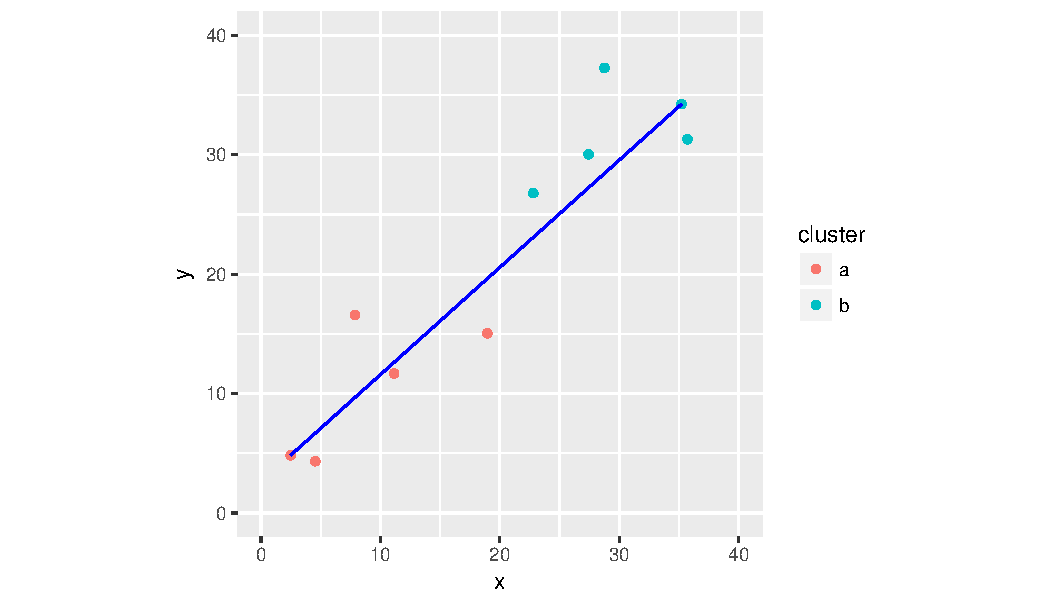
\includegraphics[width=\maxwidth]{figure/unnamed-chunk-4-1} 

\end{knitrout}

This looks good (with only 12 points).
  
\end{frame}

\begin{frame}[fragile]{Predicted survival probs}

The function we use is called
\texttt{survfit}, though actually works rather like
\texttt{predict}. 

First create a data frame of values to predict from. We'll do all
combos of ages 20 and 40, treatment and not, using
\texttt{expand.grid} to get all the combos:

 
\begin{knitrout}
\definecolor{shadecolor}{rgb}{0.969, 0.969, 0.969}\color{fgcolor}\begin{kframe}
\begin{alltt}
\hlstd{dance.new}\hlkwb{=}\hlkwd{expand.grid}\hlstd{(}\hlkwc{Treatment}\hlstd{=}\hlkwd{c}\hlstd{(}\hlnum{0}\hlstd{,}\hlnum{1}\hlstd{),}\hlkwc{Age}\hlstd{=}\hlkwd{c}\hlstd{(}\hlnum{20}\hlstd{,}\hlnum{40}\hlstd{))}
\hlstd{dance.new}
\end{alltt}
\begin{verbatim}
##   Treatment Age
## 1         0  20
## 2         1  20
## 3         0  40
## 4         1  40
\end{verbatim}
\end{kframe}
\end{knitrout}


Then run \texttt{survfit}. Actual predictions via \texttt{summary}
(next page):

 
\begin{knitrout}
\definecolor{shadecolor}{rgb}{0.969, 0.969, 0.969}\color{fgcolor}\begin{kframe}
\begin{alltt}
\hlstd{s}\hlkwb{=}\hlkwd{survfit}\hlstd{(dance.1,}\hlkwc{newdata}\hlstd{=dance.new)}
\end{alltt}
\end{kframe}
\end{knitrout}


\end{frame}

\begin{frame}[fragile]{The predictions}

One prediction \emph{for each time} for each combo of age and treatment:

{\footnotesize
 
\begin{knitrout}
\definecolor{shadecolor}{rgb}{0.969, 0.969, 0.969}\color{fgcolor}\begin{kframe}
\begin{alltt}
\hlkwd{summary}\hlstd{(s)}
\end{alltt}
\begin{verbatim}
## Call: survfit(formula = dance.1, newdata = dance.new)
## 
##  time n.risk n.event survival1 survival2 survival3 survival4
##     1     12       1  8.76e-01  9.98e-01  1.00e+00     1.000
##     2     11       2  3.99e-01  9.89e-01  9.99e-01     1.000
##     4      8       1  1.24e-01  9.76e-01  9.99e-01     1.000
##     5      7       1  2.93e-02  9.60e-01  9.98e-01     1.000
##     7      6       1 2.96e-323  1.70e-04  6.13e-01     0.994
##     8      5       1  0.00e+00  1.35e-98  2.99e-06     0.862
##    10      4       1  0.00e+00  0.00e+00  3.61e-20     0.593
##    11      2       1  0.00e+00  0.00e+00  0.00e+00     0.000
##    12      1       1  0.00e+00  0.00e+00  0.00e+00     0.000
\end{verbatim}
\begin{alltt}
\hlkwd{t}\hlstd{(dance.new)}
\end{alltt}
\begin{verbatim}
##           [,1] [,2] [,3] [,4]
## Treatment    0    1    0    1
## Age         20   20   40   40
\end{verbatim}
\end{kframe}
\end{knitrout}
}

\texttt{dance.new} transposed (flipped around) shows which combo the
four lists of survival probabilities belong to.
  
\end{frame}

\begin{frame}[fragile]{Conclusions from predicted probs}

  \begin{itemize}
  \item Older women more likely to be still dancing than younger women
    (compare ``profiles'' for same treatment group).
  \item Effect of treatment seems to be to increase prob of still dancing (compare ``profiles'' for same age for treatment group vs.\ not)
  \item Would be nice to see this on a graph.
  \end{itemize}
  
\end{frame}

\begin{frame}[fragile]{Plotting survival probabilities}
  
  \begin{itemize}
  \item I like package \texttt{survminer} with function \texttt{ggsurvplot}:
    
\begin{knitrout}
\definecolor{shadecolor}{rgb}{0.969, 0.969, 0.969}\color{fgcolor}\begin{kframe}
\begin{alltt}
\hlkwd{library}\hlstd{(survminer)}
\hlstd{g}\hlkwb{=}\hlkwd{ggsurvplot}\hlstd{(s)}
\end{alltt}
\end{kframe}
\end{knitrout}
  \end{itemize}
  
\end{frame}

\begin{frame}[fragile]{The plot}
  
\begin{knitrout}
\definecolor{shadecolor}{rgb}{0.969, 0.969, 0.969}\color{fgcolor}\begin{kframe}
\begin{alltt}
\hlstd{g}
\end{alltt}
\end{kframe}
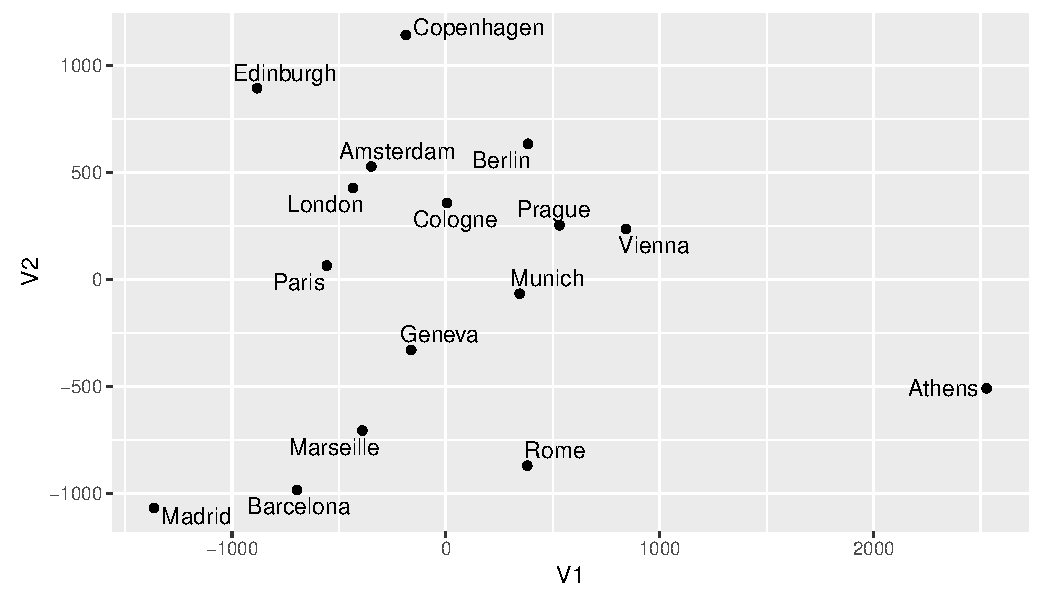
\includegraphics[width=\maxwidth]{figure/unnamed-chunk-9-1} 

\end{knitrout}

\begin{small}
\begin{tabular}{rrr}
  Stratum& Age& Treatment \\
  \hline
  1 & 20 & no\\
  2 & 20 & yes\\
  3 & 40 & no\\
  4 & 40 & yes\\
  \hline
\end{tabular}  
\end{small}
  
\end{frame}

\begin{frame}[fragile]{Discussion}
%  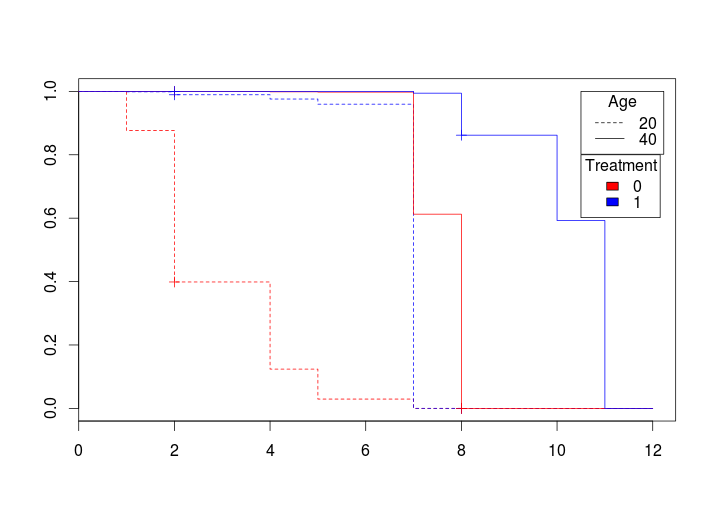
\includegraphics[width=2in]{dance-2}

  
  \begin{itemize}
  \item Survivor curve farther to the right is better (better chance
    of surviving longer).
  \item Best is age 40 with treatment, worst age 20 without.
  \item Appears to be:
    \begin{itemize}
    \item age effect (40 better than 20)
    \item treatment effect (treatment better than not)
    \end{itemize}
  \item In analysis, treatment effect only marginally significant.
  \end{itemize}

\end{frame}



\begin{frame}[fragile]{A more realistic example: lung cancer}


\begin{itemize}
\item When you
load in an R package, get data sets to illustrate 
functions in the package. 
\item One such is \texttt{lung}. Data
set measuring survival in patients with advanced lung cancer. 
\item Along with survival time, number of ``performance scores''
  included, measuring how well patients can perform daily
  activities.
\item Sometimes high good, but sometimes bad!
\item Variables below,
  from the help file data set (\texttt{?lung}).
\end{itemize}
\end{frame}

\begin{frame}[fragile]{The variables}

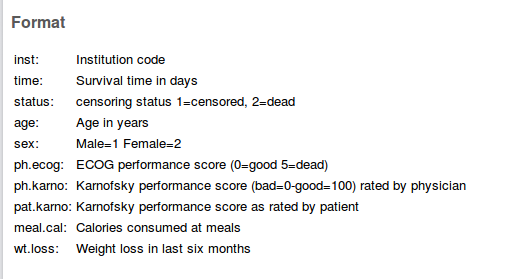
\includegraphics[width=\textwidth]{lung-cancer-data}  

  
\end{frame}

\begin{frame}[fragile]{Uh oh, missing values}
  
  \begin{scriptsize}
\begin{knitrout}
\definecolor{shadecolor}{rgb}{0.969, 0.969, 0.969}\color{fgcolor}\begin{kframe}
\begin{alltt}
\hlkwd{head}\hlstd{(lung,}\hlnum{12}\hlstd{)}
\end{alltt}
\begin{verbatim}
##    inst time status age sex ph.ecog ph.karno pat.karno meal.cal wt.loss
## 1     3  306      2  74   1       1       90       100     1175      NA
## 2     3  455      2  68   1       0       90        90     1225      15
## 3     3 1010      1  56   1       0       90        90       NA      15
## 4     5  210      2  57   1       1       90        60     1150      11
## 5     1  883      2  60   1       0      100        90       NA       0
## 6    12 1022      1  74   1       1       50        80      513       0
## 7     7  310      2  68   2       2       70        60      384      10
## 8    11  361      2  71   2       2       60        80      538       1
## 9     1  218      2  53   1       1       70        80      825      16
## 10    7  166      2  61   1       2       70        70      271      34
## 11    6  170      2  57   1       1       80        80     1025      27
## 12   16  654      2  68   2       2       70        70       NA      23
\end{verbatim}
\end{kframe}
\end{knitrout}
  \end{scriptsize}
  
\end{frame}

\begin{frame}[fragile]{Remove any obs with any missing values}
  

  
\begin{knitrout}
\definecolor{shadecolor}{rgb}{0.969, 0.969, 0.969}\color{fgcolor}\begin{kframe}
\begin{alltt}
\hlstd{lung} \hlopt \hlkwd{na.omit}\hlstd{()} \hlkwb{->} \hlstd{lung.complete}
\hlstd{lung.complete} \hlopt \hlkwd{select}\hlstd{(meal.cal}\hlopt{:}\hlstd{wt.loss)} \hlopt \hlkwd{head}\hlstd{(}\hlnum{12}\hlstd{)}
\end{alltt}
\begin{verbatim}
##    meal.cal wt.loss
## 2      1225      15
## 4      1150      11
## 6       513       0
## 7       384      10
## 8       538       1
## 9       825      16
## 10      271      34
## 11     1025      27
## 15     2600      60
## 17     1150      -5
## 18     1025      22
## 19      238      10
\end{verbatim}
\end{kframe}
\end{knitrout}
  
\end{frame}

\begin{frame}[fragile]{Model 1: use everything}

{\scriptsize  
 
\begin{knitrout}
\definecolor{shadecolor}{rgb}{0.969, 0.969, 0.969}\color{fgcolor}\begin{kframe}
\begin{alltt}
\hlkwd{head}\hlstd{(lung.complete)}
\end{alltt}
\begin{verbatim}
##   inst time status age sex ph.ecog ph.karno pat.karno meal.cal wt.loss
## 2    3  455      2  68   1       0       90        90     1225      15
## 4    5  210      2  57   1       1       90        60     1150      11
## 6   12 1022      1  74   1       1       50        80      513       0
## 7    7  310      2  68   2       2       70        60      384      10
## 8   11  361      2  71   2       2       60        80      538       1
## 9    1  218      2  53   1       1       70        80      825      16
\end{verbatim}
\end{kframe}
\end{knitrout}

}

\begin{knitrout}
\definecolor{shadecolor}{rgb}{0.969, 0.969, 0.969}\color{fgcolor}\begin{kframe}
\begin{alltt}
\hlstd{resp}\hlkwb{=}\hlkwd{with}\hlstd{(lung.complete,}\hlkwd{Surv}\hlstd{(time,status}\hlopt{==}\hlnum{2}\hlstd{))}
\hlstd{lung.1}\hlkwb{=}\hlkwd{coxph}\hlstd{(resp}\hlopt{~}\hlstd{age}\hlopt{+}\hlstd{sex}\hlopt{+}\hlstd{ph.ecog}\hlopt{+}\hlstd{ph.karno}\hlopt{+}\hlstd{pat.karno}\hlopt{+}
               \hlstd{meal.cal}\hlopt{+}\hlstd{wt.loss,}\hlkwc{data}\hlstd{=lung.complete)}
\end{alltt}
\end{kframe}
\end{knitrout}


\end{frame}

\begin{frame}[fragile]{\texttt{summary} of model 1: too tiny to see!}

{\tiny  
 
\begin{knitrout}
\definecolor{shadecolor}{rgb}{0.969, 0.969, 0.969}\color{fgcolor}\begin{kframe}
\begin{alltt}
\hlkwd{summary}\hlstd{(lung.1)}
\end{alltt}
\begin{verbatim}
## Call:
## coxph(formula = resp ~ age + sex + ph.ecog + ph.karno + pat.karno + 
##     meal.cal + wt.loss, data = lung.complete)
## 
##   n= 167, number of events= 120 
## 
##                 coef  exp(coef)   se(coef)      z Pr(>|z|)   
## age        1.080e-02  1.011e+00  1.160e-02  0.931  0.35168   
## sex       -5.536e-01  5.749e-01  2.016e-01 -2.746  0.00603 **
## ph.ecog    7.395e-01  2.095e+00  2.250e-01  3.287  0.00101 **
## ph.karno   2.244e-02  1.023e+00  1.123e-02  1.998  0.04575 * 
## pat.karno -1.207e-02  9.880e-01  8.116e-03 -1.488  0.13685   
## meal.cal   2.835e-05  1.000e+00  2.594e-04  0.109  0.91298   
## wt.loss   -1.420e-02  9.859e-01  7.766e-03 -1.828  0.06748 . 
## ---
## Signif. codes:  0 '***' 0.001 '**' 0.01 '*' 0.05 '.' 0.1 ' ' 1
## 
##           exp(coef) exp(-coef) lower .95 upper .95
## age          1.0109     0.9893    0.9881    1.0341
## sex          0.5749     1.7395    0.3872    0.8534
## ph.ecog      2.0950     0.4773    1.3479    3.2560
## ph.karno     1.0227     0.9778    1.0004    1.0455
## pat.karno    0.9880     1.0121    0.9724    1.0038
## meal.cal     1.0000     1.0000    0.9995    1.0005
## wt.loss      0.9859     1.0143    0.9710    1.0010
## 
## Concordance= 0.653  (se = 0.031 )
## Rsquare= 0.155   (max possible= 0.998 )
## Likelihood ratio test= 28.16  on 7 df,   p=0.0002053
## Wald test            = 27.5  on 7 df,   p=0.0002711
## Score (logrank) test = 28.31  on 7 df,   p=0.0001929
\end{verbatim}
\end{kframe}
\end{knitrout}
}

\end{frame}

\begin{frame}[fragile]{Overall significance}
 

The three tests of overall significance:

 
\begin{knitrout}
\definecolor{shadecolor}{rgb}{0.969, 0.969, 0.969}\color{fgcolor}\begin{kframe}
\begin{alltt}
\hlstd{s}\hlkwb{=}\hlkwd{summary}\hlstd{(lung.1)}
\hlkwd{rbind}\hlstd{(s}\hlopt{$}\hlstd{logtest,s}\hlopt{$}\hlstd{waldtest,s}\hlopt{$}\hlstd{sctest)}
\end{alltt}
\begin{verbatim}
##          test df       pvalue
## [1,] 28.16471  7 0.0002052811
## [2,] 27.50000  7 0.0002711044
## [3,] 28.31331  7 0.0001929209
\end{verbatim}
\end{kframe}
\end{knitrout}

All strongly significant. \emph{Something} predicts survival.  

\end{frame}

\begin{frame}[fragile]{Coefficients for model 1}
  
{\footnotesize  
 
\begin{knitrout}
\definecolor{shadecolor}{rgb}{0.969, 0.969, 0.969}\color{fgcolor}\begin{kframe}
\begin{alltt}
\hlstd{s}\hlopt{$}\hlstd{coefficients}
\end{alltt}
\begin{verbatim}
##                    coef exp(coef)     se(coef)          z    Pr(>|z|)
## age        1.080338e-02 1.0108619 0.0115998987  0.9313337 0.351681000
## sex       -5.536181e-01 0.5748661 0.2015855722 -2.7463179 0.006026834
## ph.ecog    7.395321e-01 2.0949551 0.2249867714  3.2870027 0.001012598
## ph.karno   2.243783e-02 1.0226914 0.0112317607  1.9977122 0.045747870
## pat.karno -1.207386e-02 0.9879987 0.0081162309 -1.4876191 0.136851382
## meal.cal   2.834683e-05 1.0000283 0.0002593848  0.1092848 0.912976585
## wt.loss   -1.420024e-02 0.9859001 0.0077662937 -1.8284443 0.067482902
\end{verbatim}
\end{kframe}
\end{knitrout}
}

  \begin{itemize}
  \item Model as a whole significant (strongly)
  \item \texttt{sex} and
\texttt{ph.ecog} definitely significant
\item \texttt{age}, \texttt{pat.karno} and
\texttt{meal.cal} definitely not
\item  others in
between
\item Take out the three variables that are definitely not
significant, and try again.
  \end{itemize}


\end{frame}


\begin{frame}[fragile]{Model 2 (edited)}

{\footnotesize  
 
\begin{knitrout}
\definecolor{shadecolor}{rgb}{0.969, 0.969, 0.969}\color{fgcolor}\begin{kframe}
\begin{alltt}
\hlstd{lung.2}\hlkwb{=}\hlkwd{update}\hlstd{(lung.1,.}\hlopt{~}\hlstd{.}\hlopt{-}\hlstd{age}\hlopt{-}\hlstd{pat.karno}\hlopt{-}\hlstd{meal.cal)}
\hlkwd{summary}\hlstd{(lung.2)}\hlopt{$}\hlstd{coefficients}
\end{alltt}
\begin{verbatim}
##                 coef exp(coef)    se(coef)         z    Pr(>|z|)
## sex      -0.57088076 0.5650276 0.198842401 -2.871021 0.004091480
## ph.ecog   0.84466049 2.3271876 0.218644264  3.863172 0.000111924
## ph.karno  0.01787711 1.0180379 0.010887199  1.642030 0.100583796
## wt.loss  -0.01204774 0.9880245 0.007495345 -1.607363 0.107974751
\end{verbatim}
\end{kframe}
\end{knitrout}
}
  
  \begin{itemize}
  \item Take out \texttt{ph.karno} and \texttt{wt.loss} as well.
  \end{itemize}
  
\end{frame}

\begin{frame}[fragile]{Model 3, and last}


{\footnotesize

 
\begin{knitrout}
\definecolor{shadecolor}{rgb}{0.969, 0.969, 0.969}\color{fgcolor}\begin{kframe}
\begin{alltt}
\hlstd{lung.3}\hlkwb{=}\hlkwd{update}\hlstd{(lung.2,.}\hlopt{~}\hlstd{.}\hlopt{-}\hlstd{ph.karno}\hlopt{-}\hlstd{wt.loss)}
\hlkwd{summary}\hlstd{(lung.3)}\hlopt{$}\hlstd{coefficients}
\end{alltt}
\begin{verbatim}
##               coef exp(coef)  se(coef)         z     Pr(>|z|)
## sex     -0.5100991 0.6004361 0.1968998 -2.590652 0.0095794186
## ph.ecog  0.4825185 1.6201497 0.1323160  3.646714 0.0002656157
\end{verbatim}
\end{kframe}
\end{knitrout}
}

%$%$

\begin{itemize}
\item Both variables strongly significant.
\item Effect on survival time:
  \begin{itemize}
  \item Higher value of \texttt{sex} (female) has \emph{negative} effect
    on event (death).
  \item Higher value of \texttt{ph.ecog} has \emph{positive} effect on death.
  \item i.\ e.\ being female or having lower \texttt{ph.ecog} score has
    positive effect on survival.
  \end{itemize}
\item Picture?
\end{itemize}
  
\end{frame}

\begin{frame}[fragile]{Comparing full model with final one}
  
  \begin{itemize}
  \item We took more than one $x$ out at once, so should check that
    removing all those $x$'s was OK:
    
\begin{knitrout}
\definecolor{shadecolor}{rgb}{0.969, 0.969, 0.969}\color{fgcolor}\begin{kframe}
\begin{alltt}
\hlkwd{anova}\hlstd{(lung.3,lung.1)}
\end{alltt}
\begin{verbatim}
## Analysis of Deviance Table
##  Cox model: response is  resp
##  Model 1: ~ sex + ph.ecog
##  Model 2: ~ age + sex + ph.ecog + ph.karno + pat.karno + meal.cal + wt.loss
##    loglik  Chisq Df P(>|Chi|)
## 1 -498.38                    
## 2 -494.03 8.6825  5    0.1224
\end{verbatim}
\end{kframe}
\end{knitrout}
\item Two models are equally good, so prefer smaller, simpler one:
  taking all those other variables out was fine.
  \end{itemize}
  
\end{frame}

\begin{frame}[fragile]{Plotting survival probabilities}

  \begin{itemize}
  \item Create new data frame of values to predict for, then predict:
  \end{itemize}

{\footnotesize
  
 
\begin{knitrout}
\definecolor{shadecolor}{rgb}{0.969, 0.969, 0.969}\color{fgcolor}\begin{kframe}
\begin{alltt}
\hlstd{lung.new}\hlkwb{=}\hlkwd{expand.grid}\hlstd{(}\hlkwc{sex}\hlstd{=}\hlkwd{c}\hlstd{(}\hlnum{1}\hlstd{,}\hlnum{2}\hlstd{),}\hlkwc{ph.ecog}\hlstd{=}\hlnum{0}\hlopt{:}\hlnum{3}\hlstd{)}
\hlstd{lung.new}
\end{alltt}
\begin{verbatim}
##   sex ph.ecog
## 1   1       0
## 2   2       0
## 3   1       1
## 4   2       1
## 5   1       2
## 6   2       2
## 7   1       3
## 8   2       3
\end{verbatim}
\begin{alltt}
\hlstd{s}\hlkwb{=}\hlkwd{survfit}\hlstd{(lung.3,}\hlkwc{newdata}\hlstd{=lung.new)}
\end{alltt}
\end{kframe}
\end{knitrout}
  
}
 
\end{frame}


\begin{frame}[fragile]{The plot}

 
\begin{knitrout}
\definecolor{shadecolor}{rgb}{0.969, 0.969, 0.969}\color{fgcolor}\begin{kframe}
\begin{alltt}
\hlkwd{ggsurvplot}\hlstd{(s)}
\end{alltt}
\end{kframe}
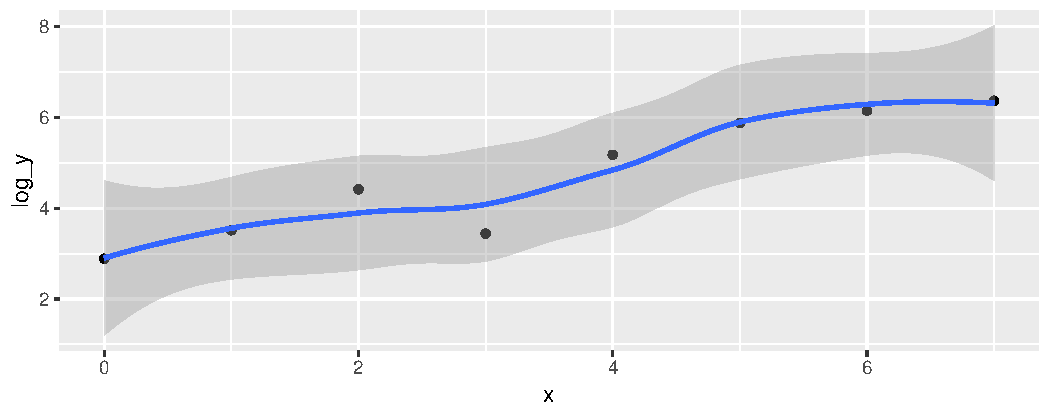
\includegraphics[width=\maxwidth]{figure/unnamed-chunk-22-1} 

\end{knitrout}
  
  
\end{frame}


\begin{frame}[fragile]{Discussion of survival curves}

  \begin{itemize}
  \item Best survival is yellow curve, stratum 2, females with
    (\texttt{ph.ecog}) score 0.
    \item Next best: dark green, stratum 4, females with score 1, and
      red, stratum 1, males score 0.
    \item Worst: purple, stratum 7, males score 3.
      \item For any given \texttt{ph.ecog} score, females have better
        predicted survival than males.
      \item For both genders, a lower score associated with better
        survival.
  \item \texttt{sex} coeff in model 3 negative, so being higher
    \texttt{sex} value (female) goes with \emph{less} hazard of dying.
  \item \texttt{ph.ecog} coeff in model 3 positive, so higher
    \texttt{ph.ecog} score goes with \emph{more} hazard of dying
  \item Two coeffs about same size, so being male rather than female
    corresponds to 1-point increase in \texttt{ph.ecog} score. Note
    how survival curves come in 3 pairs plus 2 odd.
  \end{itemize}

\end{frame}


\begin{frame}[fragile]{Martingale residuals for this model}
  
\begin{knitrout}
\definecolor{shadecolor}{rgb}{0.969, 0.969, 0.969}\color{fgcolor}\begin{kframe}
\begin{alltt}
\hlkwd{ggcoxdiagnostics}\hlstd{(lung.3)}\hlopt{+}\hlkwd{geom_smooth}\hlstd{(}\hlkwc{se}\hlstd{=F)}
\end{alltt}


{\ttfamily\noindent\itshape\color{messagecolor}{\#\# `geom\_smooth()` using method = 'loess'}}\end{kframe}
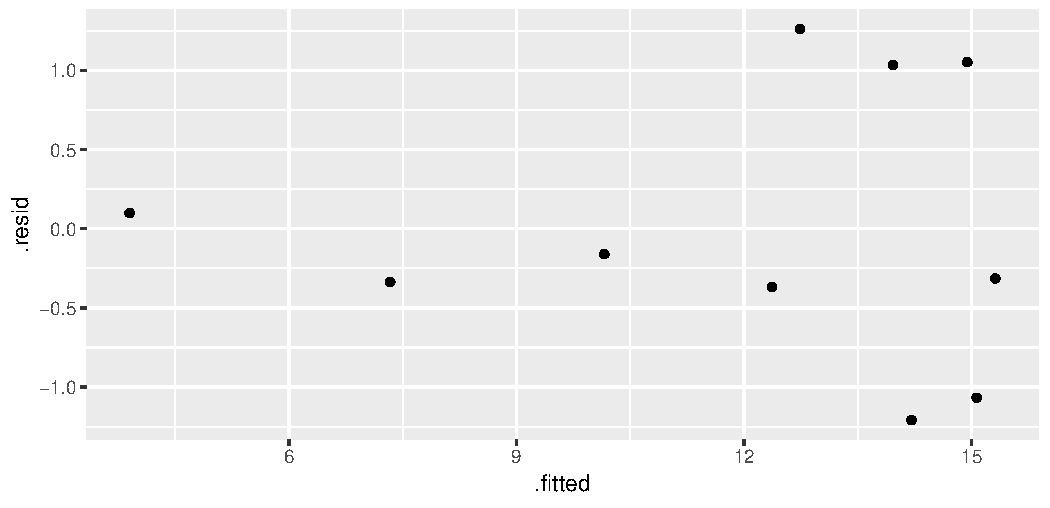
\includegraphics[width=\maxwidth]{figure/unnamed-chunk-23-1} 

\end{knitrout}

No problems here.
  
\end{frame}


\begin{frame}[fragile]{When the Cox model fails}
  \begin{itemize}
  \item Invent some data where survival is best at middling age, and
    worse at high \emph{and} low age:

\begin{knitrout}
\definecolor{shadecolor}{rgb}{0.969, 0.969, 0.969}\color{fgcolor}\begin{kframe}
\begin{alltt}
\hlstd{age}\hlkwb{=}\hlkwd{seq}\hlstd{(}\hlnum{20}\hlstd{,}\hlnum{60}\hlstd{,}\hlnum{5}\hlstd{)}
\hlstd{survtime}\hlkwb{=}\hlkwd{c}\hlstd{(}\hlnum{10}\hlstd{,}\hlnum{12}\hlstd{,}\hlnum{11}\hlstd{,}\hlnum{21}\hlstd{,}\hlnum{15}\hlstd{,}\hlnum{20}\hlstd{,}\hlnum{8}\hlstd{,}\hlnum{9}\hlstd{,}\hlnum{11}\hlstd{)}
\hlstd{stat}\hlkwb{=}\hlkwd{c}\hlstd{(}\hlnum{1}\hlstd{,}\hlnum{1}\hlstd{,}\hlnum{1}\hlstd{,}\hlnum{1}\hlstd{,}\hlnum{0}\hlstd{,}\hlnum{1}\hlstd{,}\hlnum{1}\hlstd{,}\hlnum{1}\hlstd{,}\hlnum{1}\hlstd{)}
\hlstd{d}\hlkwb{=}\hlkwd{data.frame}\hlstd{(age,survtime,stat)}
\hlstd{y}\hlkwb{=}\hlkwd{with}\hlstd{(d,}\hlkwd{Surv}\hlstd{(survtime,stat))}
\end{alltt}
\end{kframe}
\end{knitrout}

\item Small survival time 15 in middle was actually censored, so would
  have been longer if observed.
  \end{itemize}
\end{frame}

\begin{frame}[fragile]{Fit Cox model}
  
  \begin{footnotesize}
\begin{knitrout}
\definecolor{shadecolor}{rgb}{0.969, 0.969, 0.969}\color{fgcolor}\begin{kframe}
\begin{alltt}
\hlstd{y.1}\hlkwb{=}\hlkwd{coxph}\hlstd{(y}\hlopt{~}\hlstd{age,}\hlkwc{data}\hlstd{=d)}
\hlkwd{summary}\hlstd{(y.1)}
\end{alltt}
\begin{verbatim}
## Call:
## coxph(formula = y ~ age, data = d)
## 
##   n= 9, number of events= 8 
## 
##        coef exp(coef) se(coef)     z Pr(>|z|)
## age 0.01984   1.02003  0.03446 0.576    0.565
## 
##     exp(coef) exp(-coef) lower .95 upper .95
## age      1.02     0.9804    0.9534     1.091
## 
## Concordance= 0.545  (se = 0.146 )
## Rsquare= 0.036   (max possible= 0.926 )
## Likelihood ratio test= 0.33  on 1 df,   p=0.5669
## Wald test            = 0.33  on 1 df,   p=0.5649
## Score (logrank) test = 0.33  on 1 df,   p=0.563
\end{verbatim}
\end{kframe}
\end{knitrout}
    
  \end{footnotesize}
  
\end{frame}

\begin{frame}[fragile]{Martingale residuals}

\begin{knitrout}
\definecolor{shadecolor}{rgb}{0.969, 0.969, 0.969}\color{fgcolor}\begin{kframe}
\begin{alltt}
\hlkwd{ggcoxdiagnostics}\hlstd{(y.1)}\hlopt{+}\hlkwd{geom_smooth}\hlstd{(}\hlkwc{se}\hlstd{=F)}
\end{alltt}


{\ttfamily\noindent\itshape\color{messagecolor}{\#\# `geom\_smooth()` using method = 'loess'}}\end{kframe}
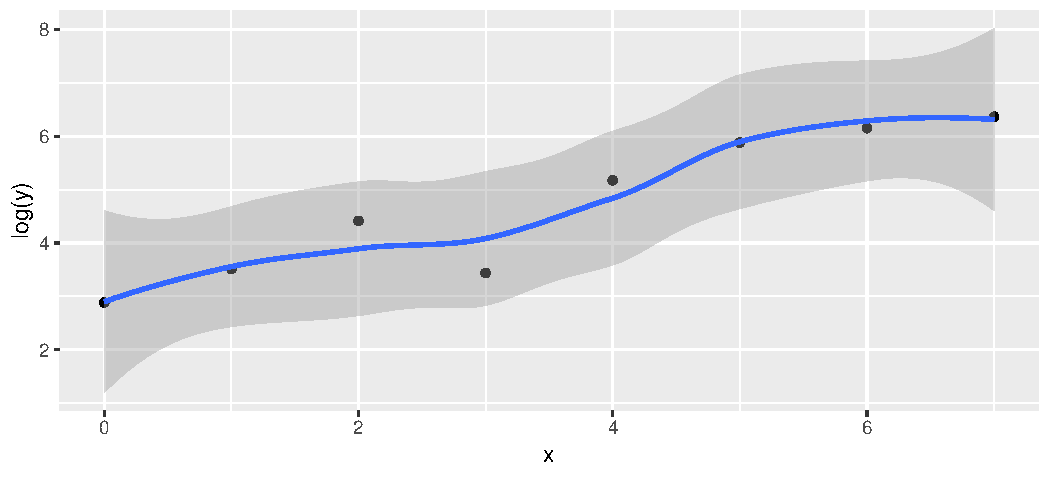
\includegraphics[width=\maxwidth]{figure/unnamed-chunk-26-1} 

\end{knitrout}

Down-and-up indicates incorrect relationship between age and
survival. Add age-squared term.
\end{frame}

\begin{frame}[fragile]{Attempt 2}
  
  \begin{footnotesize}
\begin{knitrout}
\definecolor{shadecolor}{rgb}{0.969, 0.969, 0.969}\color{fgcolor}\begin{kframe}
\begin{alltt}
\hlstd{y.2}\hlkwb{=}\hlkwd{coxph}\hlstd{(y}\hlopt{~}\hlstd{age}\hlopt{+}\hlkwd{I}\hlstd{(age}\hlopt{^}\hlnum{2}\hlstd{),}\hlkwc{data}\hlstd{=d)}
\hlkwd{summary}\hlstd{(y.2)}
\end{alltt}
\begin{verbatim}
## Call:
## coxph(formula = y ~ age + I(age^2), data = d)
## 
##   n= 9, number of events= 8 
## 
##               coef exp(coef)  se(coef)      z Pr(>|z|)  
## age      -0.380184  0.683736  0.241617 -1.573   0.1156  
## I(age^2)  0.004832  1.004844  0.002918  1.656   0.0977 .
## ---
## Signif. codes:  0 '***' 0.001 '**' 0.01 '*' 0.05 '.' 0.1 ' ' 1
## 
##          exp(coef) exp(-coef) lower .95 upper .95
## age         0.6837     1.4626    0.4258     1.098
## I(age^2)    1.0048     0.9952    0.9991     1.011
## 
## Concordance= 0.758  (se = 0.146 )
## Rsquare= 0.304   (max possible= 0.926 )
## Likelihood ratio test= 3.26  on 2 df,   p=0.1964
## Wald test            = 3.16  on 2 df,   p=0.2058
## Score (logrank) test = 3.75  on 2 df,   p=0.1536
\end{verbatim}
\end{kframe}
\end{knitrout}
  \end{footnotesize}
  
\end{frame}

\begin{frame}[fragile]{Martingale residuals this time}
  
\begin{knitrout}
\definecolor{shadecolor}{rgb}{0.969, 0.969, 0.969}\color{fgcolor}\begin{kframe}
\begin{alltt}
\hlkwd{ggcoxdiagnostics}\hlstd{(y.2)}\hlopt{+}\hlkwd{geom_smooth}\hlstd{(}\hlkwc{se}\hlstd{=F)}
\end{alltt}


{\ttfamily\noindent\itshape\color{messagecolor}{\#\# `geom\_smooth()` using method = 'loess'}}\end{kframe}
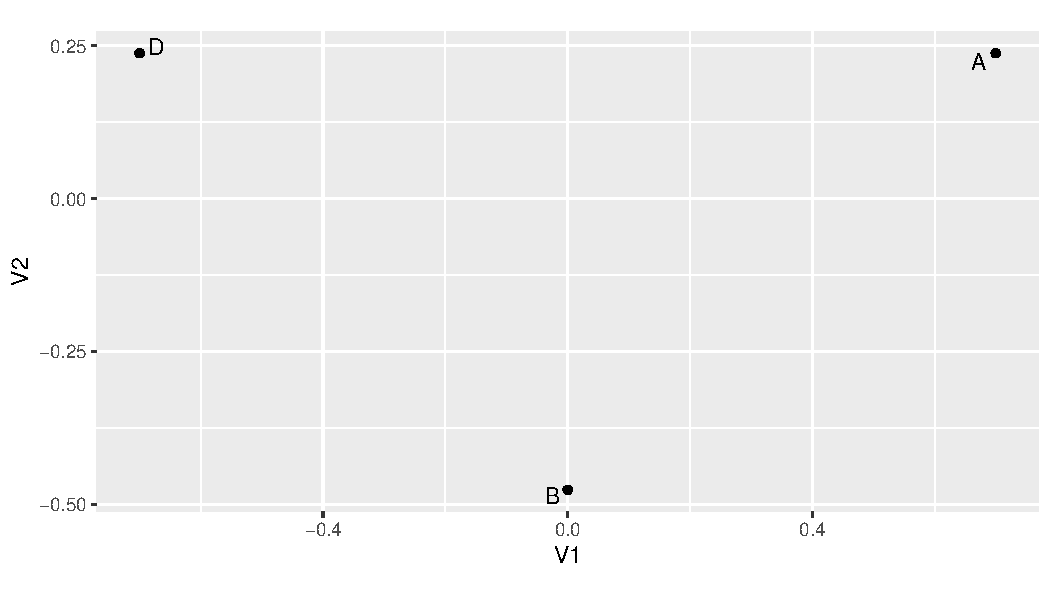
\includegraphics[width=\maxwidth]{figure/unnamed-chunk-28-1} 

\end{knitrout}

Not great, but less problematic than before.
  
\end{frame}

